\documentclass{article}
\usepackage[margin = 2.54cm]{geometry} % set margin to traditional doc

%packages
\usepackage{graphicx} % Required for inserting images
\usepackage{subcaption}
\usepackage[most]{tcolorbox} %for creating environments
\usepackage{amsmath}
\usepackage{amssymb}
\usepackage{mathtools}
\usepackage{verbatim}
\usepackage[utf8]{inputenc}
\usepackage[dvipsnames]{xcolor} %for importing multiple colors
\usepackage{hyperref} %for creating links to different sections

\linespread{1.2} %controlling line spread

%define colors i like
\definecolor{myTeal}{RGB}{0,128,128}
\definecolor{myGreen}{RGB}{34,170,34}
\definecolor{mySapphire}{RGB}{15,82,186}
\definecolor{myEmerald}{RGB}{50.4, 130, 90}

%create math environments, can add [section] or [subsection] to add index counter based on sections/subsections
\newtheorem{define}{Definition}
\newtheorem{prop}{Proposition}
\newtheorem{thm}{Theorem}
\newtheorem{question}{Question}
\newtheorem{lemma}{Lemma}

%setup colored box environment for each math env above
\tcolorboxenvironment{define}{
    enhanced, colframe=myTeal!50!teal, colback=myTeal!10,
    arc=5mm, lower separated=false, fonttitle=\bfseries
}
\tcolorboxenvironment{prop}{
    enhanced, colframe=myGreen!50!black, colback=myGreen!15,
    arc=5mm, lower separated=false, fonttitle=\bfseries
}
\tcolorboxenvironment{thm}{
    enhanced, colframe=mySapphire!50!mySapphire, colback=mySapphire!15,
    arc=5mm, lower separated=false, fonttitle=\bfseries
}
\tcolorboxenvironment{question}{
    enhanced, colframe=blue!50!black, colback=blue!10,
    arc=5mm, lower separated=false, fonttitle=\bfseries
}
\tcolorboxenvironment{lemma}{
    enhanced, colframe=myEmerald!50!myEmerald, colback=myEmerald!10,
    arc=5mm, lower separated=false, fonttitle=\bfseries
}

%setup hyperlink within pdf
\hypersetup{
    colorlinks=true,
    linkcolor=blue,
    filecolor=magenta,      
    urlcolor=cyan,
    pdftitle={Overleaf Example},
    pdfpagemode=FullScreen,
}

%common command (add to template)
%general
\newcommand{\FF}{\mathbb{F}}
\newcommand{\NN}{\mathbb{N}}
\newcommand{\ZZ}{\mathbb{Z}}
\newcommand{\QQ}{\mathbb{Q}}
\newcommand{\RR}{\mathbb{R}}
\newcommand{\CC}{\mathbb{C}}

\newcommand{\Id}{\textmd{Id}} %identity
\newcommand{\lcm}{\textmd{lcm}}
\DeclarePairedDelimiter{\abs}{\lvert}{\rvert}
\DeclarePairedDelimiter{\norm}{\lVert}{\rVert}
\DeclarePairedDelimiter{\paran}{(}{)}%paranthesis
\DeclarePairedDelimiter{\bracket}{\langle}{\rangle}

%algebra
\newcommand{\Gal}{\textmd{Gal}}
\newcommand{\Aut}{\textmd{Aut}}
\newcommand{\End}{\textmd{End}}
\newcommand{\Coker}{\textmd{Coker}}
\newcommand{\Hom}{\textmd{Hom}}
\newcommand{\Nil}{\textmd{Nil}}

%analysis
\newcommand{\Vol}{\textmd{Vol}}

%complex
\newcommand{\Real}{\textmd{Re}}
\newcommand{\Imag}{\textmd{Im}} %can also be used for Image
\newcommand{\Res}{\textmd{Res}}

%lie algebra
\newcommand{\gl}{\mathfrak{gl}}

\title{Phys 103 HW2}
\author{Zih-Yu Hsieh}

\begin{document}
\maketitle

\section{}
\begin{question}\label{q1}
    Consider an underdamped oscillator. Technically, because the amplitude decreases, the motion is not periodic and there is thus no period. We can, however, something that's enough like the period that we often just call it "the period".
    \begin{itemize}
        \item[(a)] If the oscillator starts at $x(0)=0$ (but with some initial velocity), show that subsequent zeroes are located at $t=\frac{n\pi}{w_1}$, $n \in \ZZ$. Defining the period as the amount of time to get two zeroes thus gives $\frac{2\pi}{w_1}$.
        \item[(b)] Againg setting $x(0)=0$, show that the local maxima in $x(t)$ do not occur at $t=\frac{(2n+1/2)\pi}{w_1}$; the maxima do not occur a quarter period after a zero, as would be the case for sinusoidal motion. On the other hand, show that the time between successive maxima is $\frac{2\pi}{w_1}$; defining the period as the amount of time between successive local maxima thus gives $\frac{2\pi}{w_1}$ as before. 
    \end{itemize}
\end{question}

\textbf{Pf:}

\subsection*{(a)}
Given the oscillator has the motion $x(t)=Ae^{-\beta t}\cos(w_1t-\phi)$, since $x(0) = A\cos(\phi)=0$, WLOG, can guess $\phi = \frac{\pi}{2}$ (if its $n\pi +\frac{\pi}{2}$, one can always change the constant $A$ accordingly). So, $x(t)=Ae^{-\beta t}\cos(w_1 t-\frac{\pi}{2})=Ae^{-\beta t}\sin(w_1 t)$ (here, assume $A>0$).

Which, if $x(t) = 0$, we have $Ae^{-\beta t}\sin(w_1 t)=0$. Since $A, e^{-\beta t}\neq 0$, we must have $\sin(w_1 t)=0$. As a result, $t = \frac{n\pi}{w_1}$ for $n \in \ZZ$. So, if the period is defined to be the amount of time to get two zeros, the period is $\frac{2\pi}{w_1}$ (since subsequent zeros apart each other with time $\frac{\pi}{w_1}$).

\subsection*{(b)}
If using the same equation $x(t)=Ae^{-\beta t}\sin(w_1t)$, to calculate where the local maxima is, we first consider up to its derivative:
\begin{equation}
    x'(t) = -A\beta e^{-\beta t}\sin(w_1 t)+Ae^{-\beta t}w_1\cos(w_1 t)
\end{equation}
Which, for any $n \in \ZZ$, if plug in $t=\frac{(2n+1/2)\pi}{w_1}$ to the derivative, we get:
\begin{align}
    x'\left(\frac{(2n+1/2)\pi}{w_1}\right) &= -Ae^{-\beta t}\left(\beta\sin\left(w_1\frac{(2n+1/2)\pi}{w_1}\right)-w_1\cos\left(w_1\frac{(2n+1/2)\pi}{w_1}\right)\right)\\
    &= -Ae^{-\beta t}\cdot \beta \neq 0
\end{align}
This shows that $t=\frac{(2n+1/2)\pi}{w_1}$ is no longer local maxima, since $x'(t)\neq 0$ at this point.

\hfil

However, if consider where $x'(t)=0$, suppose $t_0 \in [0,2\pi)$ satisfies $x'(t_0)=0$, we get the following relation:
\begin{align}
    x'(t_0)&=-Ae^{-\beta t_0}(-\beta\sin(w_1 t_0)+w_1\cos(w_1 t_0)) = 0,\quad Ae^{-\beta t_0}\neq 0\\
    &\implies -\beta\sin(w_1 t_0)+w_1\cos(w_1 t_0)=0\\
    &\implies \tan(w_1 t_0)=\frac{w_1}{\beta}
\end{align}
Hence, for any $n \in \ZZ$, $t=\frac{n\pi}{w_1}+t_0$ all satisfies $\tan(w_1 t)=\frac{w_1}{\beta}$,which are all zeros of $x'(t_0)$.

On the other hand, if consider the second derivative, we get the following:
\begin{equation}
    x''(t) = A(\beta^2-w_1^2)e^{-\beta t}\sin(w_1 t)-2A\beta w_1e^{-\beta t}\cos(w_1 t)
\end{equation}
Given that $t_0$ is local maximuj, $x''(t_0)<0$; however, for all $n\in\ZZ$, if $n$ is odd ($n=2k+1$ for some $k\in \ZZ$), the time $t=\frac{n\pi}{w_1}+t_0$ satisfies:
\begin{align}
    x''\left(\frac{n\pi}{w_1}+t_0\right)&=A(\beta^2-w_1^2)e^{-\beta t}\sin\left(w_1\frac{n\pi}{w_1}+w_1t_0\right) - 2A\beta w_1e^{-\beta t}\cos\left(w_1\frac{n\pi}{w_1}+w_1t_0\right)\\
    &= A(\beta^2-w_1^2)e^{-\beta (\frac{n\pi}{w_1}+t_0)}\sin((2k+1)\pi +w_1t_0)-2A\beta w_1e^{-\beta (\frac{n\pi}{w_1}+t_0)}\cos((2k+1)\pi +w_1t_0)\\
    &= -e^{-\beta\frac{n\pi}{w_1}}\left(A(\beta^2-w_1^2)e^{-\beta t_0}\sin(w_1t_0)-2A\beta w_1e^{-\beta t_0}\cos(w_1 t_0)\right)\\
    &= -e^{-\beta \frac{n\pi}{w_1}}\cdot x''(t_0)>0
\end{align}
Which, showing that $t=\frac{n\pi}{w_1}+t_0$ are all local minimum (since second derivatives are all positive). 

If $n$ is even instead ($n=2k$ for some $k\in\ZZ$), the above equation has no negative in the front, hence the second derivative remains negative, showing that $t=\frac{2k \pi}{w_1}+t_0$ are all local maxima.
So, any subsequent local maxima have a time difference of $\frac{2\pi}{w_1}$, showing that the period $\frac{2\pi}{w_1}$ can also be determined by the time between subsequent local maxima.

\break

\section{((b) not done)}
\begin{question}\label{q2}
    
    \hfil

    \begin{itemize}
        \item[(a)] Show that the energy $E$ of an underdamped oscillator (with $x=Ae^{-\beta t}\cos(w_1 t+\phi)$) is 
        $$E=\frac{1}{2}kA^2e^{-2\beta t}\left(1+\frac{1}{2Q}\cos\left(2w_1 t+2\phi-\arccos\frac{1}{2Q}\right)\right)$$
        \item[(b)] The overall exponential is easy to explain: the amplitude of the motion decreases as the damping dissipates energy, so the energy corresponding decays. Explain the physical origin of the cosine term.
        \item[(c)] $\frac{dE}{dt}$ tells us the rate at which the oscillator is losing energy. However, we can make a couople of improvements. First, rather than expressing the rate of energy loss as \emph{per unit time} we can also express it \emph{per oscillation}, as the oscillation itself provides a natural timescale. Similarly, rather than the absolute amount of energy lost, we can express the fractional energy loss by dividing by $E$.
        Next, the oscillatory terms are because of an actual physical effect: the energy does wobble a little throughout a cycle. If the oscillator is only weakly damped ($Q>>1$), we likely care much more about the overall decay after many cycles than about the slight wobble within each cycle. By time averaging over one period, we can do awway with the wobbles. These two together give us a dimensionless measure of how fast the oscillator loses on average. Show that
        $$-\left<\frac{1}{E}\frac{dE}{d\tilde{t}}\right>=\frac{2\pi}{Q}\left(1-\frac{1}{4Q^2}\right)^{-1/2}$$
        where $\tilde{t}=\frac{t}{2\pi/w_1}$ and the angle brackets indicate that we're averaging over a duration of $\frac{2\pi}{w_1}$. One interpretation of a "high quality" oscillator is the one that loses energy very slowly; if $Q$ is large, doubling the quality factor causes the oscillator to lose energy half as quickly.
    \end{itemize}
\end{question}

\textbf{Pf:}

\subsection*{(a)}
Recall that the elastic potential energy $U=\frac{1}{2}kx^2$, the kinetic energy is $K=\frac{1}{2}mv^2$, the natural frequency square $w_0^2=\frac{k}{m}$, and the frequency square $w_1^2=w_0^2-\beta^2$.

With $x(t)=Ae^{-\beta t}\cos(w_1t+\phi)$, we have the derivative $x'(t)=v(t)=-Ae^{-\beta t}(\beta \cos(w_1t+\phi)+w_1\sin(w_1t+\phi))$. Then plug in above, we get the energy as:
\begin{equation}
    U=\frac{1}{2}kx^2 = \frac{1}{2}kA^2e^{-2\beta t}\cos^2(w_1t+\phi)
\end{equation}
\begin{align}
    K&=\frac{1}{2}mv^2 = \frac{1}{2}mA^2e^{-2\beta t}(\beta^2\cos^2(w_1t+\phi)+w_1^2\sin^2(w_1t+\phi)+2\beta w_1\sin(w_1t+\phi)\cos(w_1t+\phi))\\
    &= \frac{1}{2}mA^2e^{-2\beta t}(w_0^2\sin^2(w_1t+\phi)+\beta^2(\cos^2(w_1t+\phi)-\sin^2(w_1t+\phi))+\beta w_1\sin(2w_1t+2\phi))\\
    &= \frac{1}{2}kA^2e^{-2\beta t}\sin^2(w_1t+\phi) + \frac{1}{2}mA^2e^{-2\beta t}(\beta^2\cos(2w_1t+2\phi)+\beta w_1\sin(2w_1t+2\phi))\\
    &=\frac{1}{2}kA^2e^{-2\beta t}\sin^2(w_1t+\phi) + \frac{1}{2}kA^2e^{-2\beta t}\cdot\frac{1}{w_0^2}\left(\beta^2\cos(2w_1t+2\phi)+\beta w_1\sin(2w_1t+2\phi)\right)
\end{align}
Recall that the linear combination of $\sin,\cos$ can be given as follow, for all $A,B\in \RR$:
\begin{equation}
    A\sin(x)+B\cos(x) = \sqrt{A^2+B^2}\cos\left(x-\arctan\left(\frac{B}{A}\right)\right)
\end{equation}
So, the kinetic energy can then be expressed as:
\begin{align}
    K&=\frac{1}{2}kA^2e^{-2\beta t}\sin^2(w_1t+\phi)+\frac{1}{2}kA^2e^{-2\beta t}\cdot\left(\frac{\beta}{w_0}\right)^2\cdot \sqrt{1+\left(\frac{w_1}{\beta}\right)^2}\cos\left(2w_1t+2\phi - \arctan\frac{w_1}{\beta}\right)\\
    &=\frac{1}{2}kA^2e^{-2\beta t}\sin^2(w_1t+\phi)+\frac{1}{2}kA^2e^{-2\beta t}\cdot\left(\frac{\beta}{w_0}\right)^2\cdot \sqrt{\frac{\beta^2+(w_0^2-\beta^2)}{\beta^2}}\cos\left(2w_1t+2\phi - \arctan\frac{\sqrt{w_0^2-\beta^2}}{\beta}\right)\\
    &= \frac{1}{2}kA^2e^{-2\beta t}\sin^2(w_1t+\phi)+\frac{1}{2}kA^2e^{-2\beta t}\cdot\left(\frac{\beta}{w_0}\right)^2\cdot \frac{w_0}{\beta}\cos\left(2w_1t+2\phi - \arccos\frac{\beta}{w_0}\right)
\end{align}
(Note: $\arctan(\sqrt{w_0^2-\beta^2}/\beta)=\arccos(\beta/w_0)$ can be derived through right triangle's side relations).

Then, the total energy is given as follow:
\begin{align}
    E = K+U &= \frac{1}{2}kA^3e^{-2\beta t}(\cos^2(w_1t+\phi)+\sin^2(w_1t+\phi)) + \frac{1}{2}kA^2e^{-2\beta t}\frac{2\beta}{2w_0}\cos\left(2w_1t+2\phi-\arccos\frac{2\beta}{2w_0}\right)\\
    &= \frac{1}{2}kA^2e^{-2\beta t}\left(1+\frac{1}{2Q}\cos\left(2w_1t+2\phi-\arccos\frac{1}{2Q}\right)\right)
\end{align}
(Note: recall that $Q=\frac{w_0}{2\beta}$, so $\frac{2\beta}{2w_0} = \frac{1}{2Q}$).

\subsection*{(b) (Not done)}

\subsection*{(c)}
Given that $\tilde{t}=\frac{t}{2\pi/w_1}$, then $\frac{dE}{d\tilde{t}} = \frac{dE}{dt}\frac{dt}{d\tilde{t}} = \frac{2\pi}{w_1}\frac{dE}{dt}$. Which, define $\phi_1 = 2\phi-\arccos\frac{1}{2Q}$, calculating the derivative, we get:
\begin{align}
    \frac{dE}{d\tilde{t}} &= \frac{2\pi}{w_1}\cdot \frac{1}{2}kA^2\left(-2\beta e^{-2\beta t}\left(1+\frac{1}{2Q}\cos\left(2w_1t+2\phi-\arccos\frac{1}{2Q}\right)\right) -\frac{w_1}{Q}e^{-2\beta t}\sin\left(2w_1t+2\phi-\arccos\frac{1}{2Q}\right)\right)\\
    &= -\frac{2\pi}{w_1}\cdot 2\beta E-\frac{2\pi}{w_1}\cdot \frac{w_1}{Q}\cdot\frac{1}{2}kA^2e^{-2\beta t}\sin\left(2w_1t+\phi_1\right)
\end{align}
Which, consider the term $-\frac{1}{E}\frac{dE}{d\tilde{t}}$, we get:
\begin{align}
    -\frac{1}{E}\frac{dE}{d\tilde{t}} &= \frac{2\pi}{w_1}\cdot 2\beta +\frac{2\pi}{w}\cdot \frac{w_1}{Q}\cdot\frac{\frac{1}{2}kA^2e^{-2\beta t}\sin(2w_1t+\phi_1)}{\frac{1}{2}kA^2e^{-2\beta t}\left(1+\frac{1}{2Q}\cos\left(2w_1t+\phi_1\right)\right)}\\
    &= \frac{2\pi}{w_1}\cdot 2\beta+\frac{2\pi}{w_1}\cdot\frac{2w_1}{2Q}\cdot\frac{\sin(2w_1t+\phi_1)}{1+\frac{1}{2Q}\cos(2w_1t+\phi_1)}
\end{align}
For the first term, taking the average over duration $\frac{2\pi}{w_1}$, we get $\frac{2\pi}{w_1}\cdot 2\beta$ (since it is a constant). For the second ter, since $u=1+\frac{1}{2Q}\cos(2w_1t+\phi_1)$ has derivative $-\frac{2w_1}{2Q}\sin(2w_1t+\phi_1)$, taking the average, we get:
\begin{align}
    \frac{1}{2\pi/w_1}\int_{t=0}^\frac{2\pi}{w_1}\frac{2\pi}{w_1}\cdot\frac{2w_1}{2Q}\cdot\frac{\sin(2w_1t+\phi_1)}{1+\frac{1}{2Q}\cos(2w_1t+\phi_1)} dt &= -\int_{t=0}^{\frac{2\pi}{w_1}}\frac{\frac{d}{dt}\left(1+\frac{1}{2Q}\cos(2w_1t+\phi_1)\right)}{1+\frac{1}{2Q}\cos(2w_1t+\phi_1)}dt\\
    &= -\ln\left(1+\frac{1}{2Q}\cos(2w_1t+\phi_1)\right)\bigg|_{0}^{\frac{2\pi}{w_1}}\\
    &= 0
\end{align}
(Note:recall that $\cos(2w_1t+\phi_1)$ has period $\frac{2\pi}{w_1}$).
 
As a result, since average can be distributed over addition, we get the following:
\begin{equation}
    -\left<\frac{1}{E}\frac{dE}{d\tilde{t}}\right>=\left<-\frac{1}{E}\frac{dE}{d\tilde{t}}\right> = \frac{2\pi}{w_1}\cdot 2\beta
\end{equation}
With $w_1 = \sqrt{w_0^2-\beta^2} = w_0\sqrt{1-\left(\frac{\beta}{w_0}\right)^2}$, and $Q=\frac{w_0}{2\beta}$, such average becomes:
\begin{equation}
    -\left<\frac{1}{E}\frac{dE}{d\tilde{t}}\right> = \frac{2\pi}{w_0\sqrt{1-\left(\frac{2\beta}{2w_0}\right)^2}}\cdot 2\beta  = \frac{2\pi}{Q}\left(1-\frac{1}{4Q^2}\right)^{-1/2}
\end{equation}

\break

\section{}
\begin{question}\label{q3}
    Consider a damped oscillator with natural frequency $w_0$ and damping constant $\beta$, driven by a force $F_0\cos(wt)$.
    \begin{itemize}
        \item[(a)] Show that the average power delivered to the oscillator by the driving force is 
        $$\bracket*{P}=m\beta w^2A^2$$
        and that the average power dissipated by the damping force is also the same.
        \item[(b)] Find the driving frequency which maximizes the power, assuming $F_0, w_0, \beta$ are all fixed.
    \end{itemize}
\end{question}

\textbf{Pf:}

If the differential equation is $\ddot x+2\beta \dot x + w_0^2x = \frac{\tilde{F_0}}{m}e^{iwt}$ (where $\tilde{F_0}=F_0e^{i\delta}$ for phase $\delta$; since $\delta=0$ here, $\tilde{F_0}=F_0$; divide by $m$ is because the initial setup for force is $m\ddot x$, the whole differential equation is divided by $m$), then the solution is $\frac{F_0/m}{(w_0^2-w^2)+2i\beta w}e^{iwt} = \frac{F_0}{m((w_0^2-w^2)^2+(2\beta w)^2)}((w_0^2-w^2)-2\beta wi)(\cos(wt)+i\sin(wt))$. Which, taken the real part as the solution (which corresponds to the solution of $F_0\cos(wt)$), we get:
\begin{equation}
    x(t) = \frac{F_0}{m((w_0^2-w^2)^2+(2\beta w)^2)}\paran*{(w_0^2-w^2)\cos(wt)+2\beta w\sin(wt)}
\end{equation}
Which, this is the stable state solution of the driven oscillator, which we can use tfor calculation. (Note: based on the expression, since the linear combination of $B\sin(wt)+C\cos(wt)=A\cos(wt+\phi)$ has amplitude $A=\sqrt{B^2+C^2}$, then $x(t)$ in fact has amplitude $A=\frac{F_0}{m\sqrt{(w_0^2-w^2)^2+(2\beta w)^2}}$).

\subsection*{(a)}
\subsubsection*{Power of Driving force:}
Under $1$-dimension, the power $P = Fv$ (where $v$ is the velocity), hence we first need to find the velocity:
\begin{equation}
    v(t)=x'(t) = \frac{F_0w}{m((w_0^2-w^2)^2+(2\beta w)^2)}(2\beta w\cos(wt)-(w_0^2-w^2)\sin(wt))
\end{equation}
Then, with driving force $F_{\textmd{drive}}(t)=F_0\cos(wt)$, the power is given by:
\begin{align}
    P_{\textmd{drive}}(t)&=F_{\textmd{drive}}(t)v(t) = \frac{F_0^2w}{m((w_0^2-w^2)^2+(2\beta w)^2)}(2\beta w\cos^2(wt)-(w_0^2-w^2)\sin(wt)\cos(wt))\\
    &=\frac{F_0^2w}{m((w_0^2-w^2)^2+(2\beta w)^2)}\paran*{2\beta w\cdot\frac{1+\cos(2wt)}{2}-\frac{w_0^2-w^2}{2}\sin(2wt)}
\end{align}
Which, notice that taking the average over period $\frac{2\pi}{w}$, since both $\cos(2wt),\sin(2wt)$ would provide an integral of $0$, the only term left is the constant (in the paranthesis, it's provided by $2\beta w \cdot \frac{1}{2}=\beta w$). Hence, the average driving power is:
\begin{equation}
    \bracket*{P_{\textmd{drive}}} = \frac{F_0^2\cdot\beta w^2}{m((w_0^2-w^2)^2+(2\beta w)^2)} = m\beta w^2\paran*{\frac{F_0}{m\sqrt{(w_0^2-w^2)^2+(2\beta w)^2}}}^2 = m\beta w^2A^2
\end{equation}

\subsubsection*{Power of Damping force:}
Recall that $\beta=\frac{b}{2m}$, and the damping force is provided by $F_{\textmd{damp}} = -bv$. Then, the power dissipated $P_{\textmd{damp}}=F_{\textmd{damp}}v = -bv^2$. Using the formula derived above, we get:
\begin{equation}
    P_{\textmd{damp}}(t)=-bv^2(t) = -b\cdot \frac{F_0^2w^2}{m^2((w_0^2-w^2)^2+(2\beta w)^2)^2}((2\beta w)^2\cos^2(wt)+(w_0^2-w^2)^2\sin^2(wt)-4\beta w(w_0^2-w^2)\sin(wt)\cos(wt))
\end{equation}
Which, recall that $\cos^2(wt)=\frac{1+\cos(2wt)}{2}$, $\sin^2(wt)=\frac{1-\cos(2wt)}{2}$, and $2\sin(wt)\cos(wt)=\sin(2wt)$. Taking the average over a time duration of $\frac{2\pi}{w}$, with integer multiples of $w$ being the frequency, $\sin(2wt),\cos(2wt)$ all provide average of $0$, then only the constant terms are left (which are the ones multiplied by $\frac{1}{2}$, in the $\cos(2wt)$ form of $\sin^2(wt)$ and $\cos^2(wt)$). Which, the average power dissipated by damping force is given by the constant in the above function:
\begin{align}
    \bracket*{P_\textmd{damp}} &= -b\cdot\frac{F_0^2w^2}{m^2((w_0^2-w^2)^2+(2\beta w)^2)^1}\paran*{\frac{(2\beta w)^2}{2}+\frac{(w_0^2-w^2)^2}{2}}\\
    &= -2m\beta w^2\cdot\frac{1}{2}\paran*{\frac{F_0}{m\sqrt{(w_0^2-w^2)^2+(2\beta w)^2}}}^2 = -m\beta w^2A^2
\end{align}
This shows that the driving and the damping force provides the power with same magnitude, but different sign, so the average power provided is still $0$ (i.e. the input energy from driving force is dissipated by the damping force).

\subsection*{(b)}
Given that the average power (of the driving force) is $m\beta w^2A^2$, the full form of the power is:
\begin{eqnarray}
    P_\textmd{ave} = m\beta w^2\cdot\frac{F_0^2}{m^2((w_0^2-w^2)^2+(2\beta w)^2)} = \frac{\beta F_0^2}{m\paran*{\paran*{\frac{w_0^2}{w}-w}^2+(2\beta)^2}}
\end{eqnarray}
Which, given that $F_0,\beta,w_0$ are all fixed (and nonzero), the above term has strictly psitive denominator. Hence, finding the maximum is equivalent to find the minimum of the denominator.

Given $\paran*{\frac{w_0^2}{w}-w}^2+(2\beta)^2$, its minimum occurs when the quadratic term is $0$. Hence, minimum occurs when $\frac{w_0^2}{w}-w=0$, $w^2=w_0^2$, or $w=\pm w_0$; and with $w>0$, we have the minimum occurs at $w=w_0$.

Finally, this shows that $P_\textmd{ave}$ has a maximum when $w=w_0$.

\break


\section{}
\begin{question}\label{q4}
    Consider an oscillator driven by a sawtooth wave:
    $$f(t)=f_0\paran*{\frac{t}{T}-\left\lfloor\frac{1}{2}+\frac{t}{T}\right\rfloor}$$
    \begin{itemize}
        \item[(a)] Sketch a sawtooth wave. What is the period?
        \item[(b)] Calculate the Fourier series for a sawtooth wave. Plot a sawtooth wave and a Fourier series approximation on the same figure, keeping enough terms in the sum to get a reasonably good approximation.
        \item[(c)] Calculate the response of an oscillator (with natural frequency $w_0$ and damping parameter $\beta$) driven by a sawtooth wave. make plots for several different choices of the dimensionless parameters $Tw_0$ and $Q$, making sure to include examples that are both on and off resonance. Qualitatively describe your result.
    \end{itemize}
\end{question}

\textbf{Pf:}
\subsection*{(a)}
\begin{figure}[h!]
    \begin{center}
        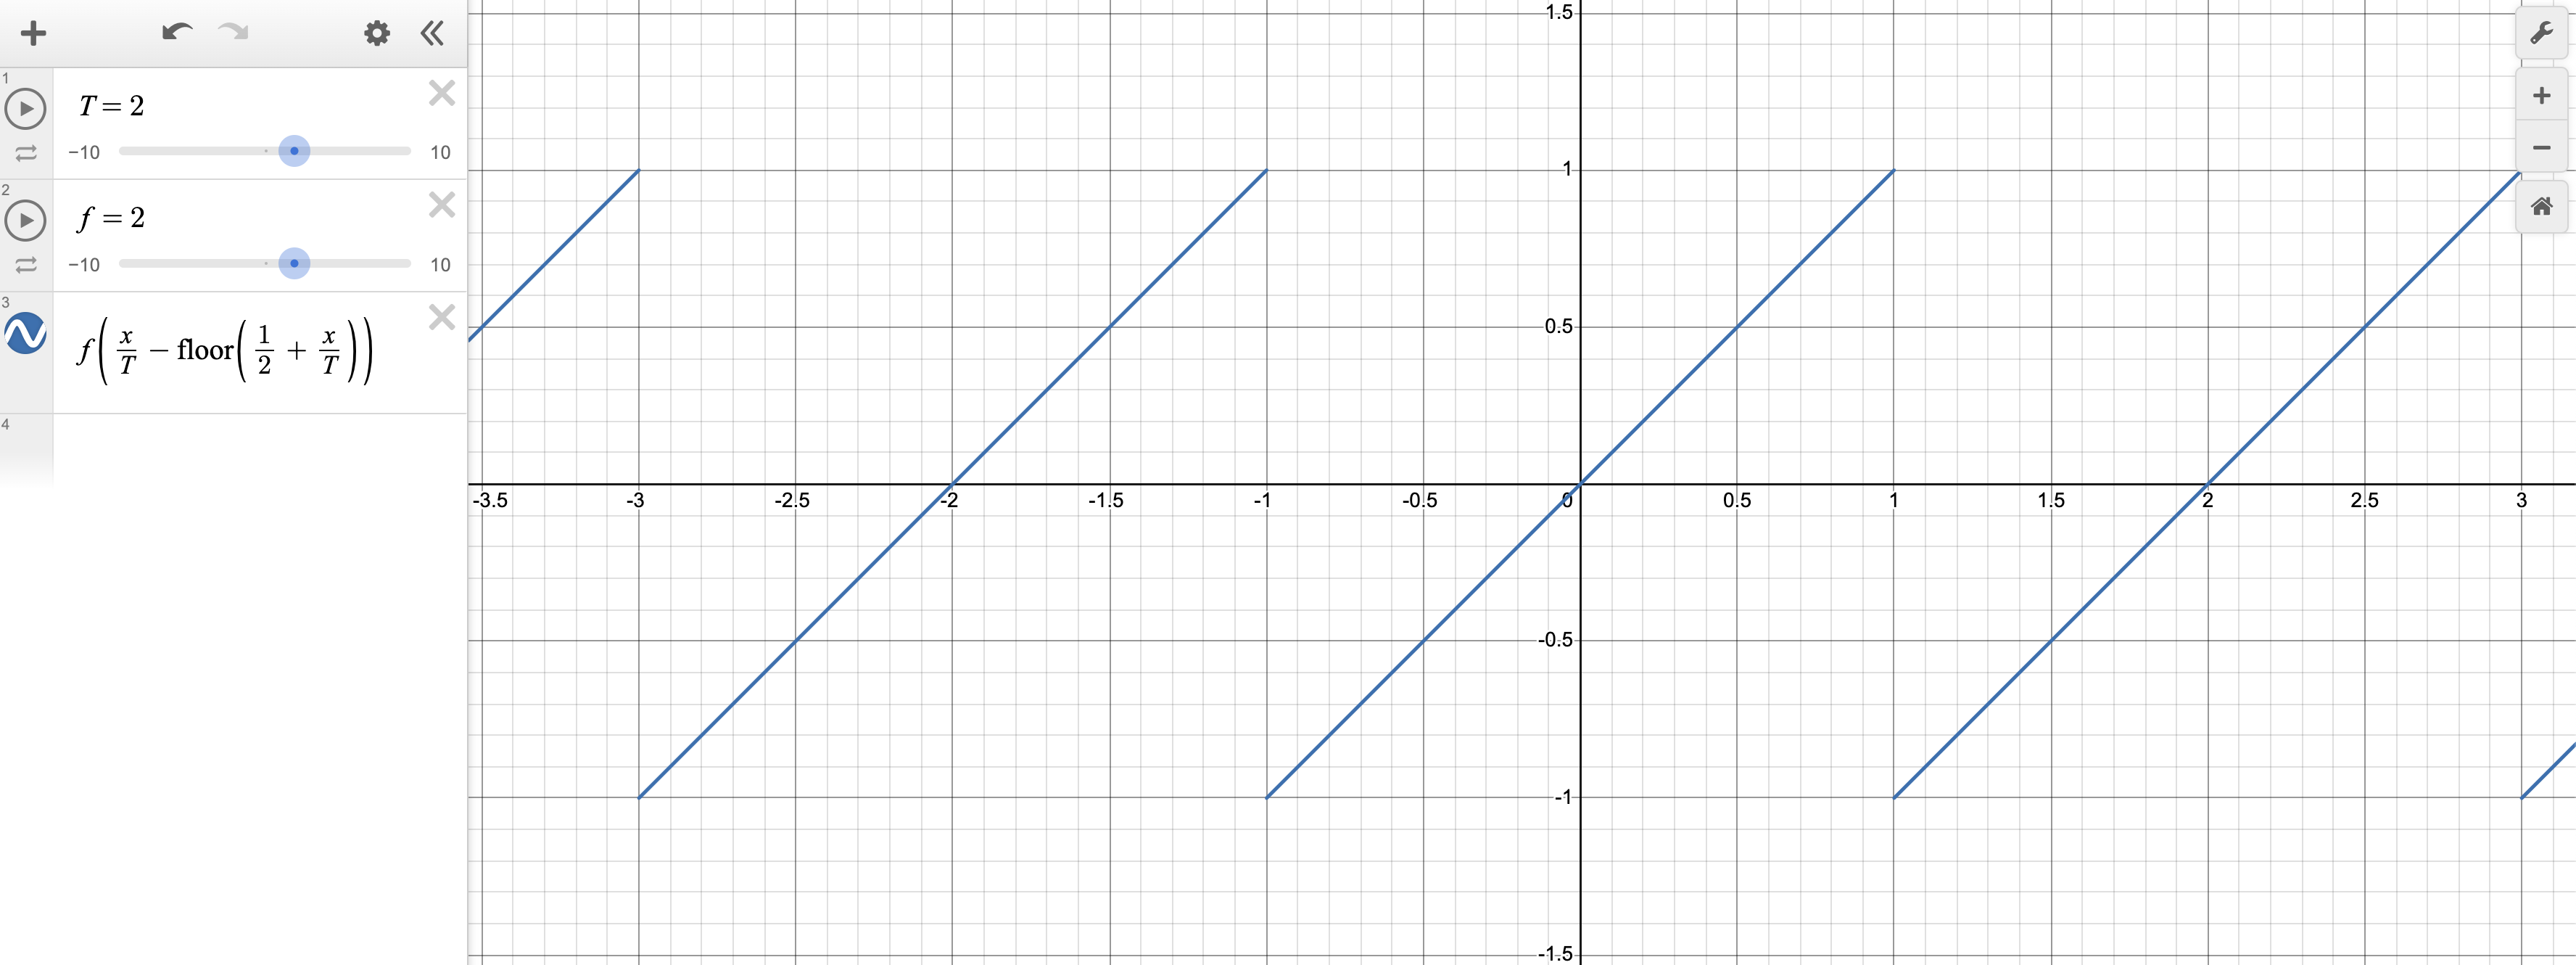
\includegraphics[width = 150mm]{sketch plot q3_a.png}
        \caption{Demonstration of the Function}
    \end{center}
\end{figure}
Based on the graph, we can conclude that the period is $T$ (also, for all $t \in \RR$, we have $f(t+T) = f_0\paran*{\frac{t+T}{T}-\left\lfloor\frac{1}{2}+\frac{t+T}{T}\right\rfloor}=f_0\paran*{1+\frac{t}{T}-\left\lfloor\frac{1}{2}+\frac{t}{T}+1\right\rfloor}$, with $\lfloor x+1\rfloor = \lfloor x\rfloor +1$, $f(t+1)=f(t)$).

\subsection*{(b)}
Within the interval $(-\frac{T}{2},\frac{T}{2})$, since $-\frac{1}{2}<\frac{t}{T}<\frac{1}{2} $, we have $0<\frac{1}{2}+\frac{t}{T}<1$, hence the floor function of this expression constantly provides $0$. Therefore, $f(t) = f_0\frac{t}{T}$.

Which, when calculating the Fourier coefficients, for all $n\in \ZZ$, we get the following:
\begin{equation}
    n=0,\quad a_0 = \frac{1}{T}\int_{-\frac{T}{2}}^\frac{T}{2}f(t)dt = \frac{1}{T}\int_{-\frac{T}{2}}^\frac{T}{2}\frac{f_0t}{T}dt = 0
\end{equation}
(Note: the above function is odd).
\begin{align}
    n\neq 0,\quad a_n &= \frac{1}{T}\int_{-\frac{T}{2}}^\frac{T}{2}f(t)e^{-i2\pi nt/T}dt = \frac{f_0}{T^2}\int_{-\frac{T}{2}}^\frac{T}{2}te^{-i2\pi nt/T}dt\\
    &=\frac{-f_0}{T\cdot i2\pi n}te^{-i2\pi nt/T}\bigg|_{-\frac{T}{2}}^\frac{T}{2} + \frac{f_0}{T\cdot i2\pi n}\int_{-\frac{T}{2}}^\frac{T}{2}e^{-i2\pi nt/T}dt\\
    &= -\frac{f_0}{i2\pi n}e^{i\pi n} +\frac{f_0}{(2\pi n)^2}e^{-i2\pi nt/T}\bigg|_{-\frac{T}{2}}^\frac{T}{2} = (-1)^{n}\frac{f_0 i}{2\pi n}
\end{align}
Hence, the Fourier Series of the function is:
\begin{align}
    f(t) = \sum_{\substack{n=-\infty\\n\neq 0}}^{\infty}\frac{(-1)^n f_0i}{2\pi n}e^{i2\pi nt/T}
\end{align}

\hfil

To plot the function, we'll convert it back to a real function. By pairing up the terms disregarding the sign, we get:
\begin{align}
    f(t)&= \sum_{n=1}^{\infty}\frac{(-1)^nf_0 i}{2\pi}\paran*{\frac{e^{i2\pi nt/T}}{n}+\frac{e^{-i2\pi nt/T}}{-n}} = \sum_{n=1}^{\infty}\frac{(-1)^nf_0 i}{n\pi}\cdot i\sin\paran*{\frac{2n\pi}{T}t}\\
    &= \sum_{n=1}^{\infty}\frac{(-1)^{n+1} f_0}{n\pi}\sin\paran*{\frac{2n\pi}{T}t}
\end{align}
Using $N=10$ as the approximation, we get the following graph:
\begin{figure}[h!]
    \begin{center}
        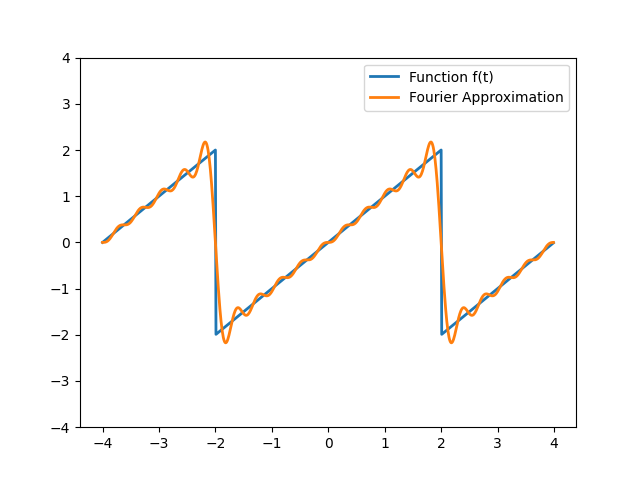
\includegraphics[width=100mm]{phys_103_hw2_q3_b.png}
        \caption{Fourier Approximation with index $n=10$}
    \end{center}
\end{figure}

Here's the provided code (source: python):

\rule{15.24cm}{0.01mm}
\begin{verbatim}
import matplotlib.pyplot as plt
import numpy as np
import math

#define constant (Note: both need to be positive)
T = 4
f_0 = 4

#define original function
def f(t):
   return f_0*(t/T - math.floor(1/2+t/T))

#define fourier series approximation, with n=10
def fourier(t):
   output = 0

   for n in range(1,11):
      output += (-1)**(n+1) * f_0 / (n* math.pi) * math.sin(2*n* math.pi * t/T)

   return output

#plot function
t = np.arange(-f_0, f_0, 0.01)

Function = []
Fourier = []
for i in range(len(t)):
   Function.append(f(t[i]))
   Fourier.append(fourier(t[i]))

plt.plot(t,Function, lw=2, label='Function f(t)')
plt.plot(t,Fourier, lw=2, label = 'Fourier Approximation')
plt.ylim(-T,T)

plt.legend()
plt.show()
\end{verbatim}

\rule{15.24cm}{0.01mm}

\subsection*{(c)}
(Note: for this part we'll focus on stable state solutions).

Recall that with periodic driven force $F_0\sin(wt)$, using methods similar to Question \ref{q3}, if develop a complex differential equation $\ddot x+2\beta \dot x+w_0^2 x=\frac{F_0}{m}e^{iwt}$ (divided by mass to get acceleration), the solution is $\tilde{x}(t)=\frac{F_0/m}{(w_0^2-w^2)+(2\beta w)i}e^{iwt} = \frac{F_0}{m((w_0^2-w^2)^2+(2\beta w)^2)}((w_0^2-w^2)-(2\beta w)i)(\cos(wt)+i\sin(wt))$. Then, if take the imaginary part, since $\Imag\paran*{\frac{F_0}{m}e^{iwt}} = \frac{F_0}{m}\sin(wt)$ (the driven force over mass), then $\Imag(\tilde{x})$ would provide a solution to our driven force. Which, we get the corresponding solution as follow:
\begin{align}
    x(t) &= \frac{F_0}{m((w_0^2-w^2)^2+(2\beta w)^2)}\paran*{(w_0^2-w^2)\sin(wt)-(2\beta w)\cos(wt)}
\end{align}
With $w = \frac{2\pi n}{T}$ for the case of Fourier Series, it can be simplified as follow:
\begin{align}
    x_n(t)&=\frac{F_n}{mw_0^4\paran*{\paran*{1-\paran*{\frac{2\pi n}{Tw_0}}^2}^2+\paran*{\frac{2\beta}{w_0}\frac{2\pi n}{Tw_0}}^2}}\cdot w_0^2\paran*{\paran*{1-\paran*{\frac{2\pi n}{Tw_0}}^2}\sin\paran*{\frac{2\pi n}{T}t}-\paran*{\frac{2\beta}{w_0}\frac{2\pi n}{Tw_0}}\cos\paran*{\frac{2\pi n}{T}t}}\\
    &= \frac{F_n}{mw_0^2\paran*{\paran*{1-\paran*{\frac{2\pi n}{Tw_0}}^2}^2+\paran*{\frac{2\pi n}{Q\cdot Tw_0}}^2}}\paran*{\paran*{1-\paran*{\frac{2\pi n}{Tw_0}}^2}\sin\paran*{\frac{2\pi n}{T}t}-\paran*{\frac{2\pi n}{Q\cdot Tw_0}}\cos\paran*{\frac{2\pi n}{T}t}}
\end{align}
Which, since the driven force is given by $f(t) = \sum_{n=1}^{\infty}\frac{(-1)^{n+1}f_0}{n\pi}\sin\paran*{\frac{2n\pi}{T}t}$, utilize linearity of differential equation, we get the following expression for the force:
\begin{align}
    x(t)=\sum_{n=1}^{\infty}x_n(t),\quad \forall n\in \NN,\ F_n = \frac{(-1)^{n+1}f_0}{n\pi}
\end{align} 
(Note: each $F_n$ represents the fourier coefficient of the $\sin(\frac{2n\pi}{T}t)$ term, since that is the "$F_0$" in the initial assumption of the sinusoidal driven force; here because each term is relatively complicated, we use some simplified notation).

For the plots, I chose $w_0=2$, $Tw_0 = \{\pi, 4\}$, and $Q=\{2,20\}$ as parameters, and $n=30$ as approximations. Here are the results:
\begin{figure}[h!]
    \centering
     \begin{subfigure}[b]{0.45\textwidth}
         \centering
         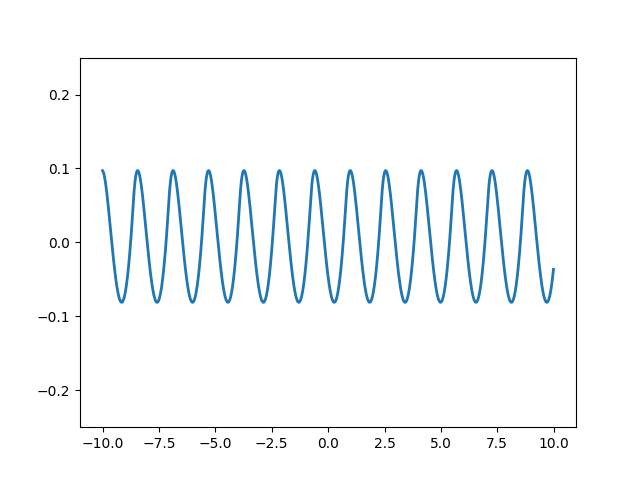
\includegraphics[width=\linewidth]{0,0.png}
         \caption{$Q=1$}
     \end{subfigure}
     \begin{subfigure}[b]{0.45\textwidth}
         \centering
         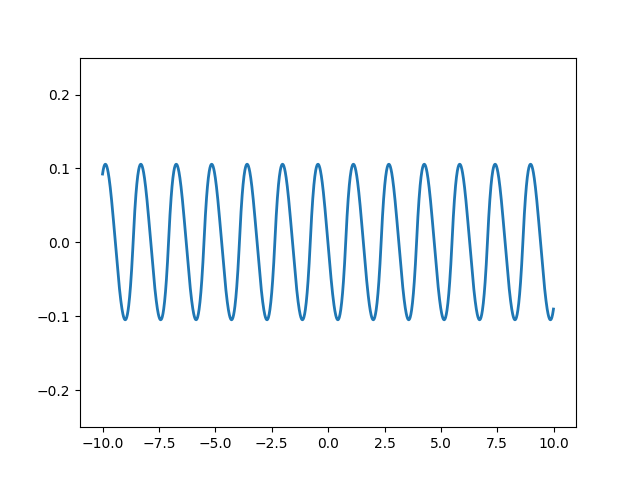
\includegraphics[width=\linewidth]{0,1.png}
         \caption{$Q=20$}
     \end{subfigure}
     \caption{When $Tw_0 = \pi$ (Not in phase with any term)}
\end{figure}

\begin{figure}[h!]
    \centering
     \begin{subfigure}[b]{0.45\textwidth}
         \centering
         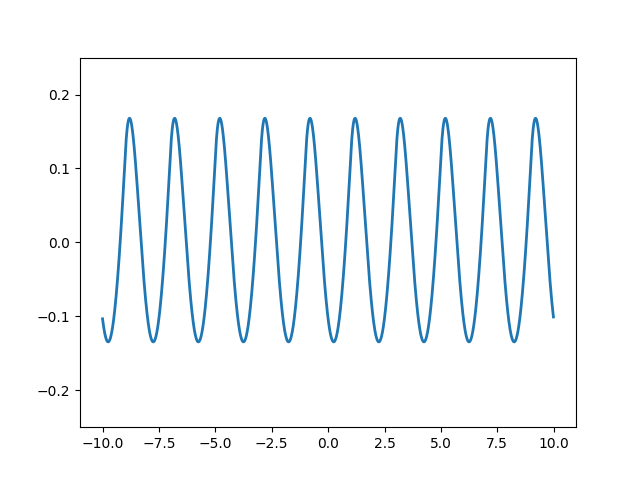
\includegraphics[width=\linewidth]{1,0.png}
         \caption{$Q=1$}
     \end{subfigure}
     \begin{subfigure}[b]{0.45\textwidth}
         \centering
         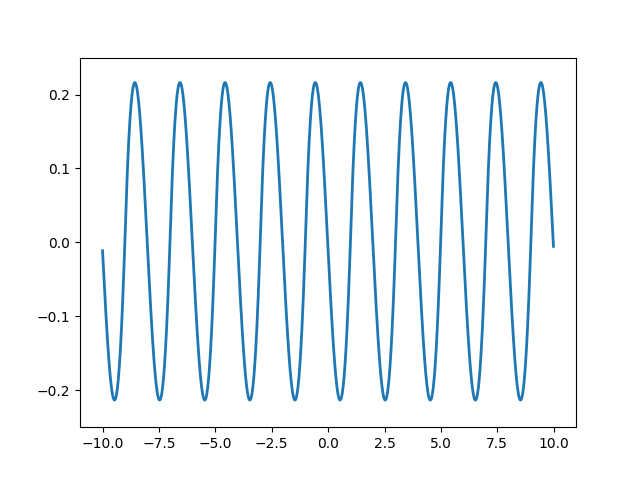
\includegraphics[width=\linewidth]{1,1.png}
         \caption{$Q=20$}
     \end{subfigure}
     \caption{When $Tw_0 = 4$ (in phase with some term)}
\end{figure}
(Note: rest of the graphs are on the next page).

So qualitatively, after getting to stable state, when quality factor $Q$ is higher, the amplitude of the system is higher (not too obvious though); on the other hand, being in phase or not affects the amplitude even more. One can see that when $Tw_0 = \pi$ (when the system is not in phase with natural frequency), the amplitude with provided constants are explicitly lower than the amplitude when $Tw_0 = 4$ (with $w_0 = 2$, the system is in phase with some force components).

\hfil

Here's the code used to generate the graphs (source: python):

\rule{15.24cm}{0.01mm}

\begin{verbatim}
import matplotlib.pyplot as plt
import numpy as np
import math

#define set of constants (Note: all need to be positive)
#fixed constant
w_0 = 2 
f_0 = 4
m=1
#array of constants
Tw_0 = [math.pi,4] #the first is never in phase, while the second always 
                    in phase with some term
Q = [1,20] #provide two different quality factors

#define the sum of solutions approximation, with n=10
def x(Tw, q, t): #here, Tw represents the Tw_0 chosen
   output = 0

   for n in range(1,31):
      w = 2* math.pi * n/(Tw)*w_0 #the frequency
      B = 1-(2 * math.pi * n/(Tw))**2 #coefficient of sin term
      C = 2* math.pi * n/(q * Tw) #coefficient of cos term

      A = (-1)**(n+1) * f_0 / (n * math.pi) * 1/(m * w_0**2 * (B**2+C**2)) #amplitude
      output += A*(B*math.sin(w*t)-C*math.cos(w*t))

   return output

#plot functions
for i in range(2): #for Tw_0
   for j in range(2): #for Q
        t = np.arange(-10, 10, 0.01)

        Tw = Tw_0[i]
        q = Q[j]

        #add X list
        X = []
        for k in range(len(t)):
            X.append(x(Tw, q, t[k]))

        #plot function on graph
        plt.plot(t,X, lw=2)
        plt.ylim(-0.25,0.25)

        plt.savefig(str(i)+','+str(j)+'.png') #save graph
        plt.clf() #clear graph
\end{verbatim}

\rule{15.24cm}{0.01mm}

\break

\section{}
\begin{question}\label{q5}
    Consider an \emph{undamped oscillator} driven exactly on resonance,
    $$\ddot x+w_0^2 x=\Real(f_0e^{9(w_0t+\delta)})$$
    If we naively plug into our formula for $C,\phi$ from lecture, we get that the amplitude is infinite, which (at least at first glance) doesn't make much sense. Solve the differential equation from scratch to get $x(t)$. Explain (with the benefit of hindsight) both how your solution is consistent with $C$ being infinite, and why (physically) the response to being driven on-resonance wit no damping has infinite amplitude.
\end{question}

\textbf{Pf:}

Temporarily, assume a solution exists, then using the 

\break

\section{}
\begin{question}\label{q6}
\end{question}

\textbf{Pf:}

\break

\section{Extra Credit}
\begin{question}\label{q7}
\end{question}

\textbf{Pf:}

\break

\end{document}